\documentclass{beamer}
\usefonttheme[onlymath]{serif}
\usepackage[T1]{fontenc}
\usepackage[utf8]{inputenc}
\usepackage[english, icelandic]{babel}
\usepackage{amsmath}
\usepackage{amssymb}
\usepackage{amsthm}
\usepackage{gensymb}
\usepackage{parskip}
\usepackage{mathtools}
\usepackage{xfrac}
\usepackage{graphicx}
\usepackage{xcolor}
\usepackage{tikz}
\usetikzlibrary{calc}
\usepackage{verbatim}
\usepackage{multicol}
\usepackage{minted}
\parskip 0pt

\DeclareMathOperator{\lcm}{lcm}
\DeclareMathOperator{\diam}{diam}
\DeclareMathOperator{\dist}{dist}
\DeclareMathOperator{\ord}{ord}
\DeclareMathOperator{\Aut}{Aut}
\DeclareMathOperator{\Inn}{Inn}
\DeclareMathOperator{\Ker}{Ker}
\DeclareMathOperator{\trace}{trace}
\DeclareMathOperator{\fix}{fix}
\DeclareMathOperator{\Log}{Log}
\newcommand\floor[1]{\left\lfloor#1\right\rfloor}
\newcommand\ceil[1]{\left\lceil#1\right\rceil}
\newcommand\abs[1]{\left|#1\right|}
\newcommand\p[1]{\left(#1\right)}
\newcommand\sqp[1]{\left[#1\right]}
\newcommand\cp[1]{\left\{#1\right\}}
\newcommand\norm[1]{\left\lVert#1\right\rVert}
\renewcommand\qedsymbol{$\blacksquare$}
\renewcommand\Im{\operatorname{Im}}
\renewcommand\Re{\operatorname{Re}}

\usetheme{Madrid}

\title{Netafræði I}
\subtitle{Óstefnd og óvigtuð net}
\author{Atli Fannar Franklín}
\date{\today}

\graphicspath{{myndir/}}

\AtBeginSection[] {
  \begin{frame}
    \frametitle{Efnisyfirlit}
    \tableofcontents[currentsection]
  \end{frame}
}


\begin{document}

\frame{\titlepage}

\section[Grunnatriði]{Grunnatriði}

\begin{frame}
\frametitle{Hvað er net?}

\begin{itemize}

\item<1-> Þið ættuð að muna eftir netum úr stærðfræðimynstrum.

\item<2-> Þetta er mengi af \textit{hnútum} sem tengdir eru með \textit{leggjum} sem liggja frá einhverjum hnút í einhvern hnút. 

\item<3-> Formlega séð er net þrennd $(V, E, \epsilon)$ þar sem $V$ er mengi hnúta, $E$ er mengi leggja og $\epsilon$ er vörpun úr $E$ í $\mathcal{P}(V)$ þ.a. $\abs{\epsilon(v)} = 1 \textrm{ eða } 2$ sem úthlutar hverjum legg \textit{endapunktum} sínum.

\item<4-> Ef hnútar hafa legg á milli sín köllum við þá nágranna. Ef tveir leggir hafa sameiginlegan endapunkt köllum við þá aðlæga. Einnig segjum að að endapunktur sé aðlægur legg sínum. Leggur með einn endapunkt kallast snara. Net þar sem engir tveir leggir hafa sömu endapunkta og hefur engar snörur kallast \textit{einfalt}.

\item<5-> Langoftast vinnum við með einföld net.

\end{itemize}

\end{frame}

\begin{frame}
\frametitle{Dæmi um net}

\begin{center}
\hspace*{-1.5cm}
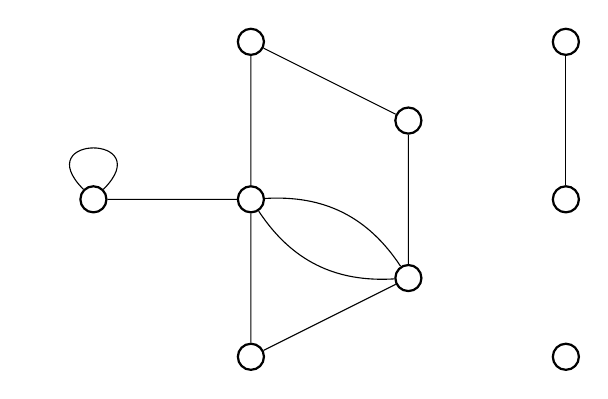
\begin{tikzpicture}

\node[draw, circle, thick] (1) at (0,0) {};
\node[draw, circle, thick] (2) at (2,0) {};
\node[draw, circle, thick] (3) at (2,2) {};
\node[draw, circle, thick] (4) at (2,-2) {};
\node[draw, circle, thick] (5) at (4,1) {};
\node[draw, circle, thick] (6) at (4,-1) {};

\node[draw, circle, thick] (7) at (6,0) {};
\node[draw, circle, thick] (8) at (6,2) {};
\node[draw, circle, thick] (9) at (6,-2) {};

\path[draw] (1) -- (2) -- (3) -- (5) -- (6) -- (4) -- (2);
\path[draw] (1) edge[in=45, out=135, looseness=10] (1);
\path[draw] (2) edge[bend left=30] (6);
\path[draw] (2) edge[bend right=30] (6);
\path[draw] (7) -- (8);

\end{tikzpicture}
\end{center}

\end{frame}

\begin{frame}
\frametitle{Vegir og rásir}

\begin{itemize}

\item<1-> Runa leggja þar sem hver leggur hefur sameiginlegan endapunkt með þeim sem kom á undan kallast vegur. Ef vegurinn byrjar og endar á sama stað köllum við hann rás. Ef við endurtökum enga hnúta köllum við veginn einfaldan. Rás er einföld ef við endurtökum enga hnúta nema þann síðasta.

\item<2-> Við segjum að tveir hnútar séu tengdir ef til er vegur milli þeirra. Samhengisþáttur í neti er þá óstækkanlegt hlutmengi hnúta sem eru allir innbyrðis tengdir.

\item<3-> Skilgreina má tré á hundrað vegu, en hér skulum við bara skilgreina það sem samanhangandi net án rása. Net án rása (sem er þá ekki nauðsynlega samanhangandi) er þá kallað skógur.

\end{itemize}

\end{frame}

\begin{frame}
\frametitle{Framsetning í tölvu}

\begin{itemize}

\item<1-> Við höfum þrjár leiðir til að tákna almenn net í tölvu (til eru einhverjar exótískari útgáfur eins og link-cut tree og heavy-light decomposition en við látum þessar þrjár duga)

\item<2-> Við höfum þá nágrannaframsetningu, fylkjaframsetningu og listaframsetningu fyrir almenn net. Notum nágrannaframsetninguna langmest. Sjáum nú þessar framsetningar fyrir netið sem við sáum áðan.

\end{itemize}

\end{frame}

\begin{frame}[fragile]
\frametitle{Nágrannaframsetning (adjacency list)}

\begin{columns}
\begin{column}{0.6\textwidth}
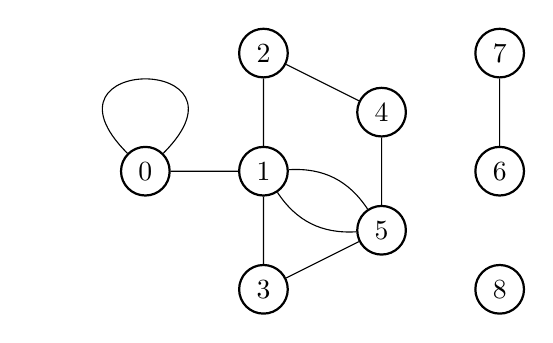
\begin{tikzpicture}[scale=0.75]

\node[draw, circle, thick] (1) at (0,0) {0};
\node[draw, circle, thick] (2) at (2,0) {1};
\node[draw, circle, thick] (3) at (2,2) {2};
\node[draw, circle, thick] (4) at (2,-2) {3};
\node[draw, circle, thick] (5) at (4,1) {4};
\node[draw, circle, thick] (6) at (4,-1) {5};

\node[draw, circle, thick] (7) at (6,0) {6};
\node[draw, circle, thick] (8) at (6,2) {7};
\node[draw, circle, thick] (9) at (6,-2) {8};

\path[draw] (1) -- (2) -- (3) -- (5) -- (6) -- (4) -- (2);
\path[draw] (1) edge[in=45, out=135, looseness=10] (1);
\path[draw] (2) edge[bend left=30] (6);
\path[draw] (2) edge[bend right=30] (6);
\path[draw] (7) -- (8);

\end{tikzpicture}
\end{column}

\begin{column}{0.4\textwidth}
\begin{verbatim}
G = [
    [0, 1],
    [2, 3, 5, 5],
    [1, 4],
    [1, 5],
    [2, 5],
    [1, 1, 3, 4],
    [7],
    [6],
    []
]
\end{verbatim}
\end{column}
\end{columns}

\vspace*{0.5cm}

\begin{itemize}

\item \verb|G| er þá listi lista og \verb|G[i]| er listi nágranna \verb|i|.

\end{itemize}

\end{frame}

\begin{frame}[fragile]
\frametitle{Fylkjaframsetning (adjacency matrix)}

\begin{columns}
\begin{column}{0.45\textwidth}
\hspace*{-1cm}
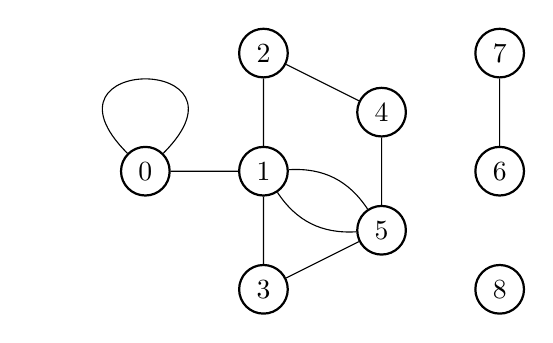
\begin{tikzpicture}[scale=0.75]

\node[draw, circle, thick] (1) at (0,0) {0};
\node[draw, circle, thick] (2) at (2,0) {1};
\node[draw, circle, thick] (3) at (2,2) {2};
\node[draw, circle, thick] (4) at (2,-2) {3};
\node[draw, circle, thick] (5) at (4,1) {4};
\node[draw, circle, thick] (6) at (4,-1) {5};

\node[draw, circle, thick] (7) at (6,0) {6};
\node[draw, circle, thick] (8) at (6,2) {7};
\node[draw, circle, thick] (9) at (6,-2) {8};

\path[draw] (1) -- (2) -- (3) -- (5) -- (6) -- (4) -- (2);
\path[draw] (1) edge[in=45, out=135, looseness=10] (1);
\path[draw] (2) edge[bend left=30] (6);
\path[draw] (2) edge[bend right=30] (6);
\path[draw] (7) -- (8);

\end{tikzpicture}
\end{column}

\begin{column}{0.55\textwidth}
\begin{verbatim}

G = [
    [1, 1, 0, 0, 0, 0, 0, 0, 0],
    [1, 0, 1, 1, 0, 2, 0, 0, 0],
    [0, 1, 0, 0, 1, 0, 0, 0, 0],
    [0, 1, 0, 0, 0, 1, 0, 0, 0],
    [0, 0, 1, 0, 0, 1, 0, 0, 0],
    [0, 2, 0, 1, 1, 0, 0, 0, 0],
    [0, 0, 0, 0, 0, 0, 0, 1, 0],
    [0, 0, 0, 0, 0, 0, 1, 0, 0],
    [0, 0, 0, 0, 0, 0, 0, 0, 0]
]
\end{verbatim}
\end{column}
\end{columns}

\vspace*{0.5cm}

\begin{itemize}

\item \verb|G| er þá listi lista og \verb|G[i][j]| er fjöldi leggja milli \verb|i| og \verb|j|.

\end{itemize}

\end{frame}

\begin{frame}[fragile]
\frametitle{Listaframsetning (edge list)}

\begin{columns}
\begin{column}{0.6\textwidth}
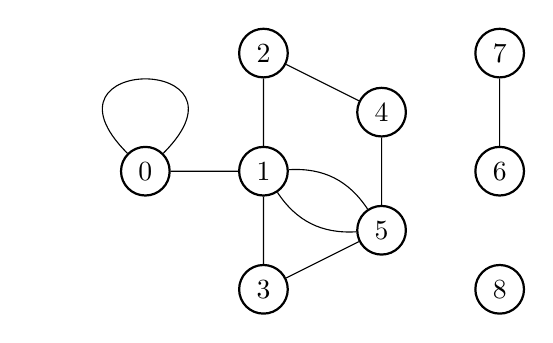
\begin{tikzpicture}[scale=0.75]

\node[draw, circle, thick] (1) at (0,0) {0};
\node[draw, circle, thick] (2) at (2,0) {1};
\node[draw, circle, thick] (3) at (2,2) {2};
\node[draw, circle, thick] (4) at (2,-2) {3};
\node[draw, circle, thick] (5) at (4,1) {4};
\node[draw, circle, thick] (6) at (4,-1) {5};

\node[draw, circle, thick] (7) at (6,0) {6};
\node[draw, circle, thick] (8) at (6,2) {7};
\node[draw, circle, thick] (9) at (6,-2) {8};

\path[draw] (1) -- (2) -- (3) -- (5) -- (6) -- (4) -- (2);
\path[draw] (1) edge[in=45, out=135, looseness=10] (1);
\path[draw] (2) edge[bend left=30] (6);
\path[draw] (2) edge[bend right=30] (6);
\path[draw] (7) -- (8);

\end{tikzpicture}
\end{column}

\begin{column}{0.4\textwidth}
\begin{verbatim}
G = [
    [0, 0],
    [0, 1],
    [1, 2],
    [1, 3],
    [1, 5],
    [1, 5],
    [2, 4],
    [3, 5],
    [4, 5],
    [6, 7]
]
\end{verbatim}
\end{column}
\end{columns}

\vspace*{0.5cm}

\begin{itemize}

\item \verb|G| er þá listi para og hvert par \verb|[i, j]| segir að til sé leggur milli \verb|i| og \verb|j| í netinu.

\end{itemize}

\end{frame}

\section[Leit í neti]{Leit í neti}

\begin{frame}
\frametitle{Netaleitir}

\begin{itemize}

\item<1-> Mörg dæmi fela það í sér að leita að einhverju í neti eða að ítra í gegnum hnúta nets. Hvernig má gera þetta?

\item<2-> Fyrir svona net (sjáum meira í næstu viku fyrir aðrar tegundir af netum) þá höfum við tvær leitar aðferðir. Við köllum þær breiddarleit (Breadth-first search, BFS) og dýptarleit (Depth-first search, DFS).

\item<3-> Bæði fela það í sér að byrja bara einhverstaðar og fara svo endurkvæmt í alla nágrannana nema þann sem maður er búinn með. Munurinn felst í því í hvaða röð þetta er gert. Í BFS hendum við nágrönnunum í biðröð en í DFS hendum við þeim á hlaða.

\item<4-> Tímaflækja reikniritanna beggja er $\mathcal{O}(V + E)$ þar sem $V$ er fjöldi hnúta og $E$ er fjöldi leggja.

\item<5-> Skoðum nú dæmi um hvernig BFS og DFS fara með ólíkum hætti í gegnum sama netið.

\end{itemize}

\end{frame}

\begin{frame}[fragile]
\frametitle{BFS}

\begin{columns}
\hspace*{1cm}
\begin{column}{0.75\textwidth}
\begin{tikzpicture}

\only<1>{\node[draw, circle, thick] (1) at (2,0) {0};}
\only<2-3>{\node[draw, circle, thick, blue, double] (1) at (2,0) {0};}
\only<4->{\node[draw, circle, thick, blue] (1) at (2,0) {0};}
\only<-2>{\node[draw, circle, thick] (2) at (2,2) {1};}
\only<-2>{\node[draw, circle, thick] (3) at (2,-2) {2};}
\only<-2>{\node[draw, circle, thick] (5) at (4,-1) {4};}
\only<3>{\node[draw, circle, thick, blue] (2) at (2,2) {1};}
\only<3-5>{\node[draw, circle, thick, blue] (3) at (2,-2) {2};}
\only<3-6>{\node[draw, circle, thick, blue] (5) at (4,-1) {4};}
\only<4-5>{\node[draw, circle, thick, blue, double] (2) at (2,2) {1};}
\only<-4>{\node[draw, circle, thick] (4) at (4,1) {3};}
\only<5-7>{\node[draw, circle, thick, blue] (4) at (4,1) {3};}
\only<6->{\node[draw, circle, thick, blue] (2) at (2,2) {1};}
\only<6>{\node[draw, circle, thick, blue, double] (3) at (2,-2) {2};}
\only<7->{\node[draw, circle, thick, blue] (3) at (2,-2) {2};}
\only<7>{\node[draw, circle, thick, blue, double] (5) at (4,-1) {4};}
\only<8->{\node[draw, circle, thick, blue] (5) at (4,-1) {4};}
\only<8-9>{\node[draw, circle, thick, blue, double] (4) at (4,1) {3};}
\only<1-8>{\node[draw, circle, thick] (6) at (6,0) {5};}
\only<9>{\node[draw, circle, thick, blue] (6) at (6,0) {5};}
\only<10->{\node[draw, circle, thick, blue] (4) at (4,1) {3};}
\only<10-11>{\node[draw, circle, thick, blue, double] (6) at (6,0) {5};}
\only<1-10>{\node[draw, circle, thick] (8) at (6,-2) {7};}
\only<1-10>{\node[draw, circle, thick] (9) at (8,0) {8};}
\only<11>{\node[draw, circle, thick, blue] (8) at (6,-2) {7};}
\only<11-12>{\node[draw, circle, thick, blue] (9) at (8,0) {8};}
\only<12>{\node[draw, circle, thick, blue, double] (8) at (6,-2) {7};}
\only<12->{\node[draw, circle, thick, blue] (6) at (6,0) {5};}
\only<13->{\node[draw, circle, thick, blue] (8) at (6,-2) {7};}
\only<13-14>{\node[draw, circle, thick, blue, double] (9) at (8,0) {8};}
\only<1-13>{\node[draw, circle, thick] (7) at (6,2) {6};}
\only<14>{\node[draw, circle, thick, blue] (7) at (6,2) {6};}
\only<15->{\node[draw, circle, thick, blue] (9) at (8,0) {8};}
\only<15>{\node[draw, circle, thick, blue, double] (7) at (6,2) {6};}
\only<16>{\node[draw, circle, thick, blue] (7) at (6,2) {6};}

\path[draw] (1) -- (2) -- (4) -- (5) -- (3) -- (1);
\path[draw] (4) -- (6) -- (8) -- (9) -- (7);
\path[draw] (6) -- (9);
\path[draw] (1) edge[bend left=30] (5);
\path[draw] (1) edge[bend right=30] (5);

\end{tikzpicture}
\end{column}

\begin{column}{0.25\textwidth}
\texttt{q = [} \\
\only<1> {
\texttt{    0\\}
}
\only<3> {
\texttt{    1,\\}
\texttt{    2,\\}
\texttt{    4\\}
}
\only<4> {
\texttt{    2,\\}
\texttt{    4\\}
}
\only<5> {
\texttt{    2,\\}
\texttt{    4,\\}
\texttt{    3\\}
}
\only<6> {
\texttt{    4,\\}
\texttt{    3\\}
}
\only<7> {
\texttt{    3\\}
}
\only<9> {
\texttt{    5\\}
}
\only<11> {
\texttt{    7,\\}
\texttt{    8\\}
}
\only<12> {
\texttt{    8\\}
}
\only<14> {
\texttt{    6\\}
}
\texttt{]}
\end{column}
\end{columns}

\end{frame}

\begin{frame}[fragile]
\frametitle{BFS útfærsla með nágrannalista}

\begin{scriptsize}
\begin{minted}{cpp}
#include<bits/stdc++.h>
using namespace std;
typedef vector<int> vi;
typedef vector<vi> vvi;

int main() {
    int n, m, a, b;
    cout << "Gefðu upp fjölda hnúta og leggja\n";
    cin >> n >> m;
    cout << "Gefðu upp m leggi (0-index)\n";
    vvi g(n, vi());
    for(int i = 0; i < m; ++i) {
        cin >> a >> b;
        g[a].push_back(b), g[b].push_back(a);
    }
    queue<int> q; vector<bool> d(n, false);
    q.push(0); d[0] = true;
    cout << "Í samhengisþætti 0 fundust:\n";
    while(!q.empty()) {
        int cur = q.front(); q.pop();
        cout << cur << '\n'; 
        for(int x : g[cur]) {
            if(d[x]) continue;
            d[x] = true; q.push(x); }}}
\end{minted}
\end{scriptsize}

\end{frame}

\begin{frame}[fragile]
\frametitle{DFS}

\begin{columns}
\hspace*{1cm}
\begin{column}{0.75\textwidth}
\begin{tikzpicture}

\only<1>{\node[draw, circle, thick] (1) at (2,0) {0};}
\only<2-3>{\node[draw, circle, thick, blue, double] (1) at (2,0) {0};}
\only<4->{\node[draw, circle, thick, blue] (1) at (2,0) {0};}
\only<1-2>{\node[draw, circle, thick] (2) at (2,2) {1};}
\only<3>{\node[draw, circle, thick, blue] (2) at (2,2) {1};}
\only<4-5>{\node[draw, circle, thick, blue, double] (2) at (2,2) {1};}
\only<6->{\node[draw, circle, thick, blue] (2) at (2,2) {1};}
\only<1-2>{\node[draw, circle, thick] (3) at (2,-2) {2};}
\only<3-13>{\node[draw, circle, thick, blue] (3) at (2,-2) {2};}
\only<14>{\node[draw, circle, thick, blue, double] (3) at (2,-2) {2};}
\only<15->{\node[draw, circle, thick, blue] (3) at (2,-2) {2};}
\only<1-4>{\node[draw, circle, thick] (4) at (4,1) {3};}
\only<5>{\node[draw, circle, thick, blue] (4) at (4,1) {3};}
\only<6-7>{\node[draw, circle, thick, blue, double] (4) at (4,1) {3};}
\only<8->{\node[draw, circle, thick, blue] (4) at (4,1) {3};}
\only<1-2>{\node[draw, circle, thick] (5) at (4,-1) {4};}
\only<3-14>{\node[draw, circle, thick, blue] (5) at (4,-1) {4};}
\only<15>{\node[draw, circle, thick, blue, double] (5) at (4,-1) {4};}
\only<16->{\node[draw, circle, thick, blue] (5) at (4,-1) {4};}
\only<1-6>{\node[draw, circle, thick] (6) at (6,0) {5};}
\only<7>{\node[draw, circle, thick, blue] (6) at (6,0) {5};}
\only<8-9>{\node[draw, circle, thick, double, blue] (6) at (6,0) {5};}
\only<10->{\node[draw, circle, thick, blue] (6) at (6,0) {5};}
\only<1-11>{\node[draw, circle, thick] (7) at (6,2) {6};}
\only<12>{\node[draw, circle, thick, blue] (7) at (6,2) {6};}
\only<13>{\node[draw, circle, thick, blue, double] (7) at (6,2) {6};}
\only<14->{\node[draw, circle, thick, blue] (7) at (6,2) {6};}
\only<1-8>{\node[draw, circle, thick] (8) at (6,-2) {7};}
\only<9>{\node[draw, circle, thick, blue] (8) at (6,-2) {7};}
\only<10>{\node[draw, circle, thick, blue, double] (8) at (6,-2) {7};}
\only<11->{\node[draw, circle, thick, blue] (8) at (6,-2) {7};}
\only<1-8>{\node[draw, circle, thick] (9) at (8,0) {8};}
\only<9-10>{\node[draw, circle, thick, blue] (9) at (8,0) {8};}
\only<11-12>{\node[draw, circle, thick, blue, double] (9) at (8,0) {8};}
\only<13->{\node[draw, circle, thick, blue] (9) at (8,0) {8};}

\path[draw] (1) -- (2) -- (4) -- (5) -- (3) -- (1);
\path[draw] (4) -- (6) -- (8) -- (9) -- (7);
\path[draw] (6) -- (9);
\path[draw] (1) edge[bend left=30] (5);
\path[draw] (1) edge[bend right=30] (5);

\end{tikzpicture}
\end{column}

\begin{column}{0.25\textwidth}
\texttt{s = [} \\
\only<1> {
\texttt{    0\\}
}
\only<3> {
\texttt{    1,\\}
\texttt{    2,\\}
\texttt{    4\\}
}
\only<4> {
\texttt{    2,\\}
\texttt{    4\\}
}
\only<5> {
\texttt{    3,\\}
\texttt{    2,\\}
\texttt{    4\\}
}
\only<6> {
\texttt{    2,\\}
\texttt{    4\\}
}
\only<7> {
\texttt{    5,\\}
\texttt{    2,\\}
\texttt{    4\\}
}
\only<8> {
\texttt{    2,\\}
\texttt{    4\\}
}
\only<9> {
\texttt{    7,\\}
\texttt{    8,\\}
\texttt{    2,\\}
\texttt{    4\\}
}
\only<10> {
\texttt{    8,\\}
\texttt{    2,\\}
\texttt{    4\\}
}
\only<11> {
\texttt{    2,\\}
\texttt{    4\\}
}
\only<12> {
\texttt{    6,\\}
\texttt{    2,\\}
\texttt{    4\\}
}
\only<13> {
\texttt{    2,\\}
\texttt{    4\\}
}
\only<14> {
\texttt{    4\\}
}
\texttt{]}
\end{column}
\end{columns}

\end{frame}

\begin{frame}[fragile]
\frametitle{DFS útfærsla með nágrannalista}

\begin{scriptsize}
\begin{minted}{cpp}
#include<bits/stdc++.h>
using namespace std;
typedef vector<int> vi;
typedef vector<vi> vvi;

int main() {
    int n, m, a, b;
    cout << "Gefðu upp fjölda hnúta og leggja\n";
    cin >> n >> m;
    cout << "Gefðu upp m leggi (0-index)\n";
    vvi g(n, vi());
    for(int i = 0; i < m; ++i) {
        cin >> a >> b;
        g[a].push_back(b), g[b].push_back(a);
    }
    stack<int> q; vector<bool> d(n, false);
    q.push(0); d[0] = true;
    cout << "Í samhengisþætti 0 fundust:\n";
    while(!q.empty()) {
        int cur = q.top(); q.pop();
        cout << cur << '\n'; 
        for(int x : g[cur]) {
            if(d[x]) continue;
            d[x] = true; q.push(x); }}}
\end{minted}
\end{scriptsize}

\end{frame}

\begin{frame}
\frametitle{Samhengisþættir}

\begin{itemize}

\item<1-> Við sjáum að þetta fer bara í gegnum einn samhengisþátt netsins.

\item<2-> Ef netið er ekki samanhangandi (s.s. hefur fleiri en einn samhengisþátt) þá þarf að halda utan um samhengisþættina og leita í hverjum fyrir sig.

\item<3-> Gera má það með union-find með því að join-a öllum aðlægum hnútum og gefur þá union-find-ið í hvaða samhengisþætti hver hnútur er.

\item<4-> Sjáum meira um þetta þegar við tölum um tengihnúta og brýr, en fyrst stutt innskot um tvíhlutanet.

\end{itemize}

\end{frame}

\section[Tvíhlutanet]{Tvíhlutanet}

\begin{frame}
\frametitle{Litun á neti}

\begin{itemize}

\item<1-> Þegar talað er um litun á neti er átt við að lita hnúta netsins þannig að engir nágrannar hafi sama lit.

\item<2-> Að finna lágmarksfjölda lita í neti er NP-vandamál svo við munum ekki skoða það hér. Jafnvel bara að skoða hvort lita megi net með 3 litum er NP-vandamál.

\item<3-> Hvort lita megi net með einum lit er ekki spennandi því það er hægt þ.þ.a.a. netið hafi enga leggi. Því er tilvikið fyrir tvo liti það sem við munum skoða. Hvenær má lita net með tveimur litum?

\item<4-> Þegar þetta er hægt má skipta hnútunum í tvo hópa svo allir leggirnir liggji milli hópa en ekki milli tveggja hnúta í sama hópnum.

\item<5-> Net þar sem þetta er hægt kallast tvíhlutanet (bipartite graph).

\end{itemize}

\end{frame}

\begin{frame}
\frametitle{Tvíhlutanet}

\begin{itemize}

\item<1-> Tvíhlutanet hafa marga þægilega eiginleika. Þið getið til dæmis reynt að sannfæra ykkur um að tvíhlutanet hafi engar rásir af odda lengd.

\item<2-> En hvernig ákvörðum við hvort net sé tvíhlutanet?

\item<3-> Við getum reynt að lita það í tveimur litum gráðugt og séð hvort við litum okkur út í horn!

\item<4-> Litum upphafspunkt bláan, nágranna hans rauða, nágranna þeirra bláa o.s.frv. og sjáum hvort það gangi upp. Göngum s.s. í gegnum netið með BFS og litum jafnóðum. Gera þarf þetta fyrir hvern samhengisþátt og er netið tvíhlutanet ef sérhver samhengisþáttur þess er það.

\item<5-> Sjáum hér útfærslu fyrir einn samhengisþátt (eða samanhangandi net)

\end{itemize}

\end{frame}

\begin{frame}[fragile]
\frametitle{Tvíhlutatékk}

\begin{scriptsize}
\begin{minted}{cpp}
#include<bits/stdc++.h>
using namespace std;
typedef vector<int> vi;
typedef vector<vi> vvi;

bool bipartite(vvi& g) {
    queue<int> q;
    q.push(0);
    vi color(g.size(), -1);
    color[0] = 0;
    while(!q.empty()) {
        int cur = q.front();
        q.pop();
        for(int x : g[cur]) {
            if(color[x] == -1) {
                color[x] = 1 - color[cur];
                q.push(x);
            } else if(color[x] == color[cur]) {
                return false;
            }
        }
    }
    return true;
}
\end{minted}
\end{scriptsize}

\end{frame}

\section[Tengihnútar og brýr]{Tengihnútar og brýr}

\begin{frame}
\frametitle{Tengihnútar og brýr}

\begin{itemize}

\item<1-> Tengihnútar (cut points) eru hnútar sem hafa þann eiginleika að ef þeir eru fjarlægðir fjölgar samhengisþáttum netsins. Brýr (bridges) eru leggir með sama eiginleika. Þeir eru því hnútar/leggir sem eru nauðsynlegir til að halda netinu samanhangandi.

\item<2-> Ef maður horfir á mynd af neti er yfirleitt frekar auðvelt að 'sjá út' hvaða hnútar eru tengihnútar og hvaða leggir eru brýr. Skoðum dæmi um þetta.

\end{itemize}

\end{frame}

\begin{frame}
\frametitle{Dæmi um tengihnúta og brýr}

\begin{center}
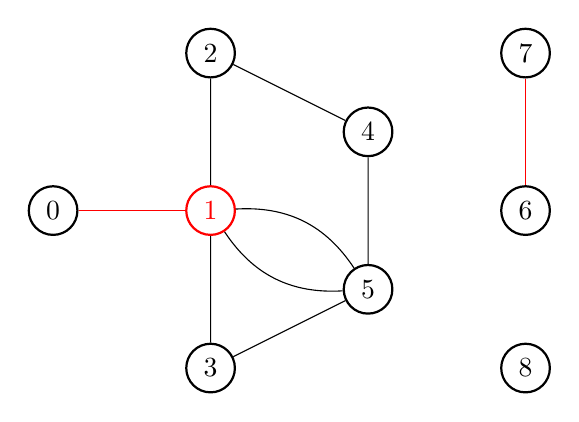
\begin{tikzpicture}
\node[draw, circle, thick] (1) at (0,0) {0};
\node[draw, circle, thick, red] (2) at (2,0) {1};
\node[draw, circle, thick] (3) at (2,2) {2};
\node[draw, circle, thick] (4) at (2,-2) {3};
\node[draw, circle, thick] (5) at (4,1) {4};
\node[draw, circle, thick] (6) at (4,-1) {5};

\node[draw, circle, thick] (7) at (6,0) {6};
\node[draw, circle, thick] (8) at (6,2) {7};
\node[draw, circle, thick] (9) at (6,-2) {8};

\path[draw] (1) edge[red] (2);
\path[draw] (2) -- (3) -- (5) -- (6) -- (4) -- (2);
\path[draw] (2) edge[bend left=30] (6);
\path[draw] (2) edge[bend right=30] (6);
\path[draw] (7) edge[red] (8);
\end{tikzpicture}
\end{center}

\end{frame}

\begin{frame}[fragile]
\frametitle{Að finna tengihnúta og brýr}

\begin{itemize}

\item<1-> En hvernig má finna þetta með tölvu?

\item<2-> Kemur í ljós að finna má þetta allt með því að fara í gegnum netið með einu DFS!

\item<3-> Þegar við löbbum í gegn með DFS geymum við fyrir hvern hnút tvær tölur, oftast kallaðar \verb|low| og \verb|num|.

\item<4-> \verb|num| geymir hvað það tók okkur mörg skref að komast í þann hnút með DFS leitinni og \verb|low| segir hvert er lægsta \verb|num| gildi sem er hægt að komast í úr þessum hnút án þess að endurtaka leggi sem við notuðum í DFS leitinni sjálfri.

\item<5-> Ef við förum í hnút $v$ á eftir hnút $u$ og við endum með að \verb|low| fyrir $v$ sé stærra en \verb|num| fyrir $u$ þá er leggurinn frá $u$ til $v$ brú því við komumst bara úr $v$ í $u$ með þeim eina legg.

\item<6-> Ef við förum í hnút $v$ á eftir hnút $u$ og við endum með að \verb|low| fyrir $v$ sé stærra en eða jafnt \verb|num| fyrir $u$ þá er $u$ tengihnútur því þá er enginn önnur leið til baka úr $v$ sem fer ekki um $u$.

\end{itemize}

\end{frame}

\begin{frame}[fragile]
\frametitle{Að reikna \texttt{num} og \texttt{low}}

\begin{itemize}

\item<1-> En hvernig reiknum við þessar tölur?

\item<2-> Í byrjun förum við bara í gegnum netið með DFS og setjum \texttt{num} útfrá því. Við látum í byrjun bara \texttt{low} vera jafnt \texttt{num} í hverjum hnút.

\item<3-> Svo ef við rekumst á legg sem við notuðum ekki í DFS-leitinni til að komast í hnútinn sem við erum stödd í uppfærum við \texttt{low} fyrir alla hnútana sem komast í þann legg.

\item<4-> Þetta virkar fyrir alla hnútana nema fyrir þann sem við byrjum í, en við tékkum bara á honum sérstaklega.

\item<5-> Skoðum nú útfærslu á þessu

\end{itemize}

\end{frame}

\begin{frame}[fragile]
\frametitle{Tengihnúta- og brúarleit útfærð}

\begin{tiny}
\begin{minted}{cpp}
#include<bits/stdc++.h>
using namespace std;
typedef vector<int> vi;
typedef vector<vi> vvi;
typedef pair<int,int> ii;
typedef vector<ii> vii;

vi low, num;
int curnum;

void dfs(vvi &g, vi &cp, vii &bri, int u, int p) {
    low[u] = num[u] = curnum++;
    int cnt = 0; bool found = false;
    for(int v : g[u]) {
        if(num[v] == -1) {
            dfs(g, cp, bri, v, u);
            low[u] = min(low[u], low[v]);
            cnt++; found |= low[v] >= num[u];
            if(low[v] > num[u]) bri.push_back(ii(u, v));
        } else if(p != v) low[u] = min(low[u], num[v]); }
  if(found && (p != -1 || cnt > 1)) cp.push_back(u); }

pair<vi,vii> cutpointsbridges(vvi &g) {
    vi cp; vii bri;
    num = vi(g.size(), -1);
    low.resize(g.size());
    curnum = 0;
    for(int i = 0; i < g.size(); ++i) {
        if(num[i] == -1) {
            dfs(g, cp, bri, i, -1);
        }
    }
    return pair<vi,vii>(cp, bri); }
\end{minted}
\end{tiny}

\end{frame}

\section[Erfið dæmi]{Erfið dæmi}

\begin{frame}
\frametitle{Fleiri NP-dæmi}

\begin{itemize}

\item<1-> Gott er að vita hvaða dæmi eru tölvunarfræðilega erfið að leysa því þá veit maður að ef þau koma upp í keppni er eitthvað skrýtið í gangi. Yfirleitt þýðir það að einhversstaðar í dæminu er eitthvað auka skilyrði gefið sem gerir dæmið leysanlegt. Gott er þá að þekkja venjulegu útgáfur dæmanna til að geta séð hvaða skilyrði eru mikilvæg.

\item<2-> Erfitt er að finna stærsta mengi hnúta sem eru allir tengdir með legg tveir og tveir (maximum clique problem)

\item<3-> Erfitt er að finna stærsta mengi hnúta sem hafa enga leggi á milli sín (maximum independent set problem), hins vegar má leysa það í tvíhlutanetum frekar hratt (sjá bók)

\item<4-> Erfitt er að finna minnsta mengi hnúta sem eru saman aðlægir öllum leggjum netsins (minimum vertex cover problem), hins vegar má leysa það í tvíhlutanetum frekar hratt (sjá bók)

\item<5-> Erfitt er að finna hvort net hafi rás/veg sem fer í gegnum hvern hnút nákvæmlega einu sinni. Hins vegar er töluvert auðveldara að finna hvort net hafi rás/veg sem fer í gegnum hvern legg nákvæmlega einu sinni (sjá bók)

\end{itemize}

\end{frame}

\end{document}